 \documentclass[a4paper,12pt, notitlepage, oneside, onecolumn]{article}
\usepackage[utf8x]{inputenc}
\usepackage[margin=3cm]{geometry}
\usepackage[]{graphicx}
\usepackage{amssymb,amsmath}
\usepackage{url}
\usepackage{hyperref}
\usepackage{array}
\usepackage{multirow}
\usepackage{float}


% Different font in captions
\newcommand{\captionfonts}{\footnotesize}

%for table caption size
\makeatletter  % Allow the use of @ in command names
\long\def\@makecaption#1#2{%
  \vskip\abovecaptionskip
  \sbox\@tempboxa{{\captionfonts #1: #2}}%
  \ifdim \wd\@tempboxa >\hsize
    {\captionfonts #1: #2\par}
  \else
    \hbox to\hsize{\hfil\box\@tempboxa\hfil}%
  \fi
  \vskip\belowcaptionskip}
\makeatother   % Cancel the effect of \makeatletter
%

\setlength{\parindent}{0pt}
% here we go...

\begin{document}
\begin{center}
{\Large{\bf Android app for dynamic traffic routing}}\\*[3mm]
Project Report\\*[5mm]
Lakesh Kansakar  and Yi Jia and Vladimir Coric\\*[3mm]
\end{center}


\begin{abstract}
In today's world time has been the most valuable asset for every person. As it is rightly said, every second counts, it is very much important to keep oneself efficient and utilize as much time as possible. People normally travel by cars and lose several hours every day because of traffic and other incidents like accidents, inefficient paths etc. In this situation, if one could know the best path to follow to reach his/her destination then it could save a lot of time. So our main motive for this project is to create an application that could provide dynamic traffic routing information. Based upon the most recent traffic information, it could provide the quickest path to the user given the source and target place and the time of the day. Mobile phones are easily accessible nowadays. Moreover, many individuals have smart phones. So, a mobile application that could actually provide this useful feature to help them find the quickest path to reach their destination will be wonderful. Our another goal is reduction of the bandwidth consumption. There are lots of services out there like google maps which provide this service. One of  the problems with these services is that you need to download the map data from their server. This will definitely consume some bandwidth which might not be desirable for people specially if you are running on low bandwidth services. This is where the concept of offline maps fits in. If we have all the map data in the phone itself, then we just need to get the information about the path. This will definitely save some bandwidth. So our overall target is to create a dynamic and bandwidth friendly routing application.
\end{abstract}

\section{Introduction}
It's always ones utmost priority to reach to his/her destination on time. However, because of traffic issues like accidents, high traffic volume, people lose several hours every day. It is possible to reach a certain destination following several paths. But it might not be feasible for a person to guess which one would be the best, which one would have less traffic and crowd. If only he/she has an application that could actually show  the best path then it would be wonderful. Further consider the scenario, lets say we have an accident at a particular place. Then it is obvious that if the person moves out at that period, then he will have to lose some time because of the accident. So, if a system could predict what the traffic condition will be like in say half an hour and tell if it would be better for this guy to move out half an hour later rather than now because of lets say traffic will be less dense, then it will be really useful.\\

The world is shifting from dekstop based applications to mobile and web based applications. Nowadays mobile phones are easily accessible. With the advent of 3G and 4G networks and performance of smart phones, it is possible to access high definition content in mobile phones. However, high volume of content requires higher bandwidth which will incur more cost to the consumer. In this situation, it would be beneficial for the person to use an application that could consume as much less bandwidth as possible and provide him all the services that he needs which is routing in our case.\\

We are actually, proposing a mobile based application that can provide dynamic routing information to the users. Based upon the recent traffic information, the service can actually provide the user with the path that will take the shortest of time to reach the destination. Based upon the speed information available at the stations or sensors, our server can actually update the cost information at regular interval of time. This makes sure that the user is provided the quickest path based upon the updated information rather than the information one year ago. We are actually planning to make the system work in real time.

\subsection{Related Work}
There are lots of sources out there that actually provide this feature in some sense; Google being the most widely used among them. Further, there are  popular services like Cloudmade which produces  APIs, rendered maps and geographic-related services like shortest path, navigation etc. However, our target is to focus on offline map data, which is provided by openstreetmaps and develop a routing service based upon the recent traffic information.

\section{Methodology}

\subsection{Architecture}

Basically as in every client-server application, our system consists of two components.

\begin{itemize}
\item Server side
\item Client side
\end{itemize}

The client side is reponsible for providing the user an interface to view the map, allow him/her to select the locations(source,destination), pick date time of the year and show the route. On the other hand the server side is reponsible for serving the routing requests from the clients. It does the bulk of processing of updating the cost of the different routes/edges based upon the current traffic information update and provide the user with the quickest path to reach his/her destination.

\begin{figure}[ht]
\begin{minipage}[b]{1.0\linewidth}
\centering
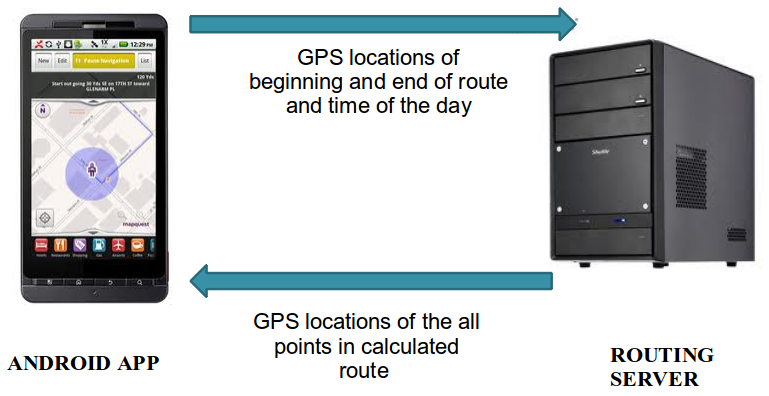
\includegraphics[scale=0.5]{architecture.png}
\caption{Basic architecture of the system}
\label{fig:architecture}
\end{minipage}
\centering
\end{figure}

\subsection{Client side}
\subsubsection{Map selection}
We have chosen openstreetmaps\cite{openstreetmap} for our offline map. OSM is open and there are lots of contributors out there who are actually adding/modifying/rectifying map information. The best part about OpenStreetMap is that it is free and general people can actually provide map information. Our other option was to use google maps. But since google doesn't allow you to have offline maps we have chosen OSM over google maps.

\subsubsection{Platform}
Out of the available platforms like iOS, Android, Symbian etc, we have chosen Android\cite{android} for our project because it is open source and there are lots of developers, contributors working on this project. Further, it's free and we don't have to pay for it. So, we have chosen this platform instead of others. Morever, Android is constantly evolving bringing in new features. Therefore, we believe that it is the best match for our objective. 

\subsubsection{Application}
Our application is a derivative of an open source application called Osmand \cite{osmand}.  As it is rightly said, it is not a good thing to reinvent the wheel, we already have this open source application osmand that actually provides most of the features that we want like offline maps, map rendering feature, interface to choose the start end destination etc. Further, it has already integrated routing services like CloudMade, Yours, OpenRouteService etc. In this situation, we found it efficient to actually add our routing service Temple on top of what it already had and use its exiting code to display the map as well as the route provided by our Temple server.\\

\begin{figure}[H]
\begin{minipage}[b]{1.0\linewidth}
\centering
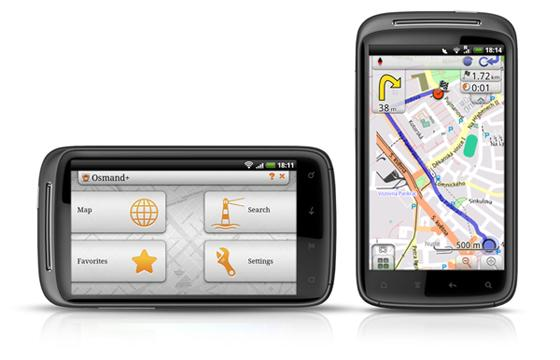
\includegraphics[scale=0.6]{osmand.jpg}
\caption{Osmand application}
\label{fig:osmand}
\end{minipage}
\centering
\end{figure}


\subsubsection{Navigation Feature}

\begin{figure}[H]
\begin{minipage}[b]{0.5\linewidth}
\centering
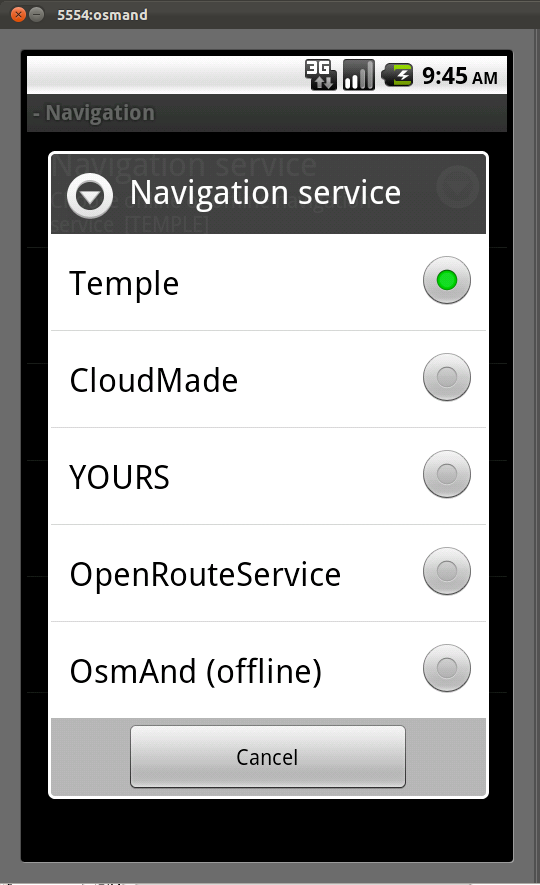
\includegraphics[scale=0.3]{navigation.png}
\caption{Temple routing service in osmand}
\label{fig:navigation}
\end{minipage}
\centering
\end{figure}
As you can see in figure \ref{fig:navigation}, Osmand  has already integrated with the routing services provided by CloudMade, YOURS, OpenRouteService as well as offline routing (which it recommends when the source and destination are far apart). So we added our own service called Temple on top of that. So, when the user chooses Temple as a navigation service, our server gets the request for the shortest route and then returns the corresponding path in the form of gps coordinates.


\subsubsection{Offline Maps}

\begin{figure}[ht]
\begin{minipage}[b]{0.5\linewidth}
\centering
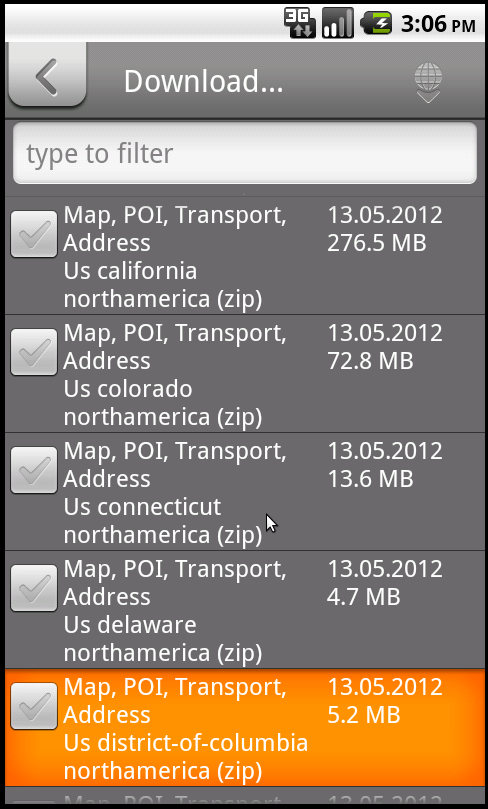
\includegraphics[scale=0.3]{offline_map_section.png}
\caption{Downloading offline maps}
\label{fig:offline_map_section}
\end{minipage}
\begin{minipage}[b]{0.5\linewidth}
\centering
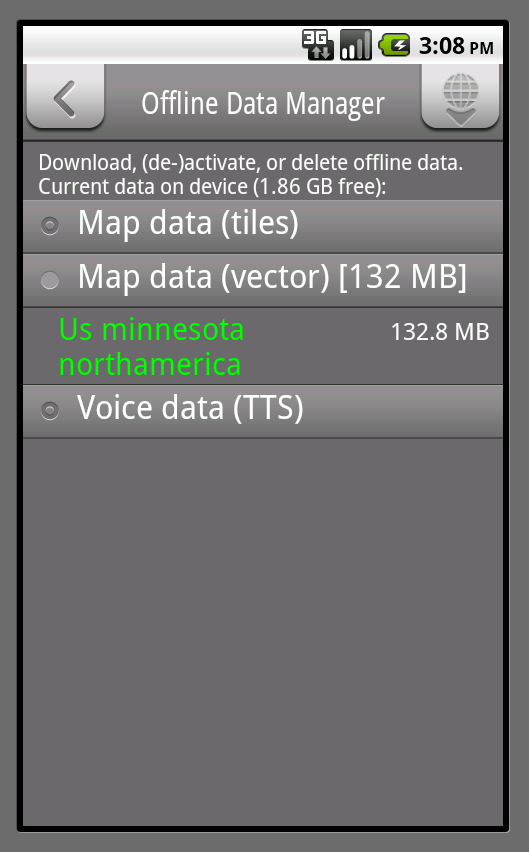
\includegraphics[scale=0.3]{offline_map_detail.png}
\caption{Installed offline maps}
\label{fig:offline_map_detail}
\end{minipage}
\end{figure}

As we had mentioned before Osmand already has this feature of offline data. It can actually fetch the map data online or use the offline data that can be downloaded once and stored in the mobile phone itself. Osmand actually has a repository from where the offline maps can be downloaded and stored in the phone. Furthermore, they have special tools that can compress the default Openstreetmap in .osm format and convert them into their own format called obf format. This format of data has comparatively less size than that of the original osm format. So, this will definitely save some bandwidth. Osmand has this option of downloading both the vector and raster form of maps.\\

\textbf{Raster maps(Tiles)}\\
These types of maps are actually images which are made up of pixels. For a particular zoom level, a set of images also called tiles display the map area. If the user needs to zoom in more then new sets of images cover the display area providing more details. Tiles actually consume more space and bandwidth\\

\textbf{Vector maps}\\
They consume comparatively less space. The map is actually represented in the form of xml. The building blocks of these type of maps basically contain nodes, ways, relations, tags etc\cite{openstreetmap_elements}. The vector maps are further compressed in binary format. Osmand has used its own binary format called osmand binary format(.obf)\cite{obf} to compress the vector maps and distribute them.


\subsubsection{Workflow}
\begin{figure}[H]
\begin{minipage}[b]{1.0\linewidth}
\centering
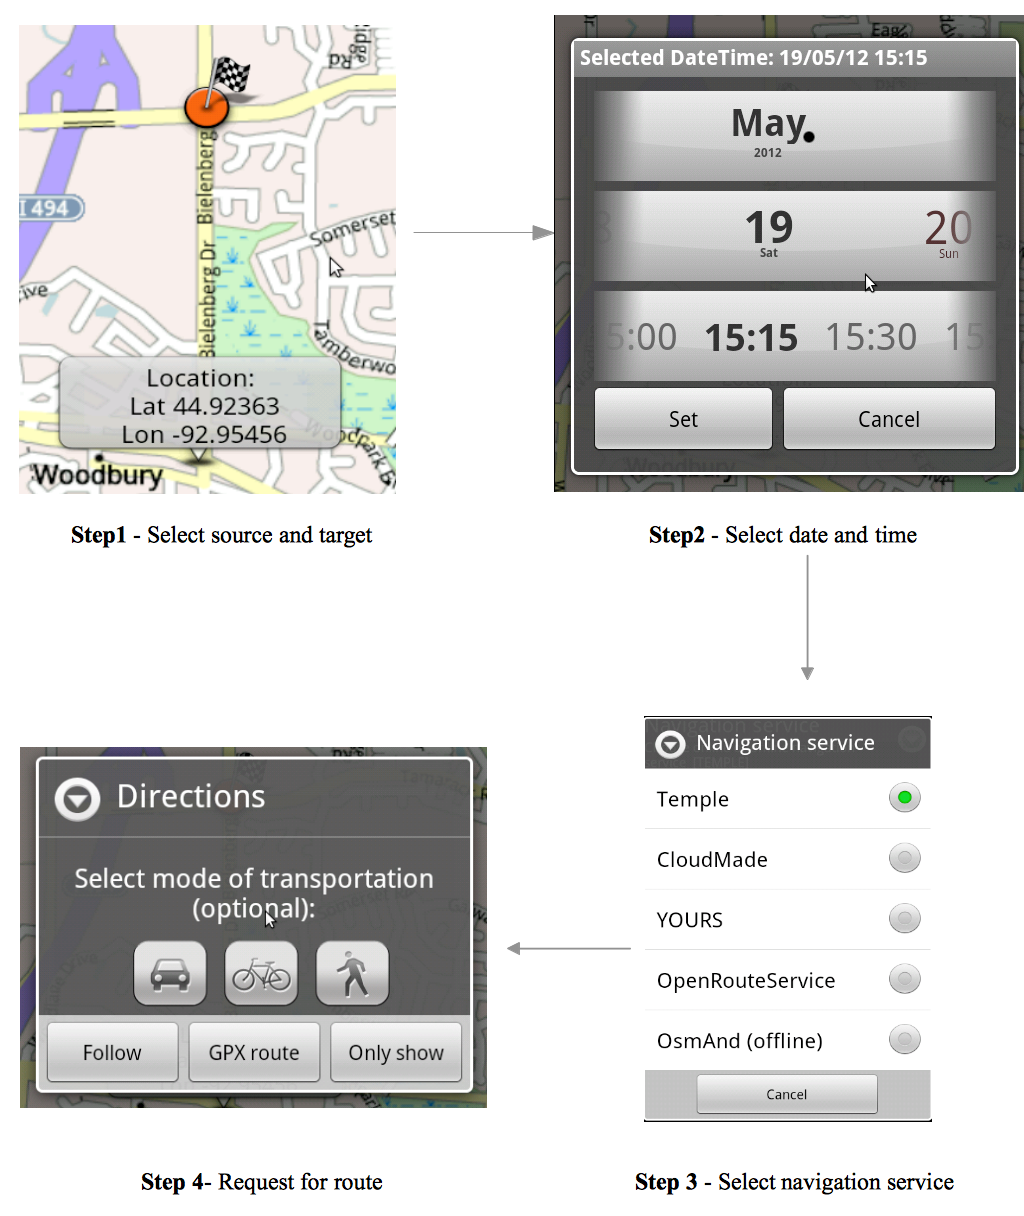
\includegraphics[scale=0.4]{workflow.png}
\caption{Workflow in the client side}
\label{fig:workflow}
\end{minipage}
\centering
\end{figure}

\begin{figure}[H]
\begin{minipage}[b]{0.5\linewidth}
\centering
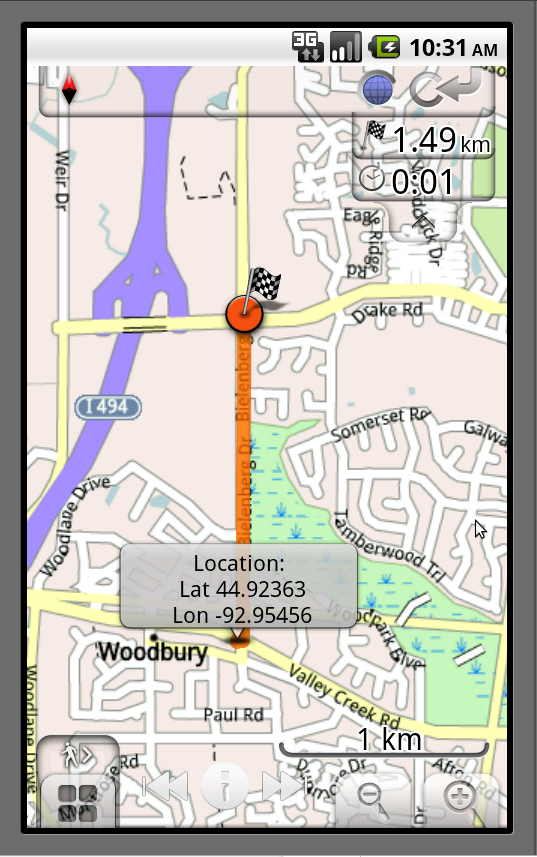
\includegraphics[scale=0.3]{route.png}
\caption{Route displayed in the client app}
\label{fig:route}
\end{minipage}
\centering
\end{figure}

The figure \ref{fig:route} shows the path displayed by our application. Given the start and end coordinates as well as the datetime, the client requests our Temple server to get the quickest path. The server then returns the path in the form of gps locations in a special file format called gpx format. Our application then plots the route given in the gpx file. Further, as we have mentioned osmand already had this feature to plot the path from a gpx file. So, we used that feature to display our path as well. Currently Osmand has lots more features like voice navigation, choosing routes based upon walking, car or bicycle. It's good to have all these features already built in. However, for our basic purpose we are only using navigation by car. In future, we can actually exploit all these other features that osmand provides.

\subsubsection{Data Exchange}
Our service currently providing the routing services resides in a web server powered by Apache at Temple's internal server accessible at data.ist.temple.edu. To actually pass information from our client side to the server, we make a standard http GET request.\\

So lets say our start location's latitude and longitude information is 43.0298,-93.1286. Similarly let the end location's latitude and longitude be given by 43.1598,-93.2349.
The datetime be 2005-04-12. Then the corresponding \textbf{GET} request will be.\\

\textbf{GET} http://data.ist.temple.edu/routes.php{?}start\_latitude=43.0298\&start\_longitude=-93.1286\&end\_latitude=43.1598\&end\_longitude=-93.2349\&date\_time=2005-04-12\\

As you can see all the parameters like start and end locations are passed as standard \textbf{GET} parameters. The server can then read these parameters and return the quickest path to the client. We had discussed that the server exchanges the quickest path information in the form of gpx\cite{gpx} file.

\begin{figure}[H]
\begin{minipage}[b]{1.0\linewidth}
\centering
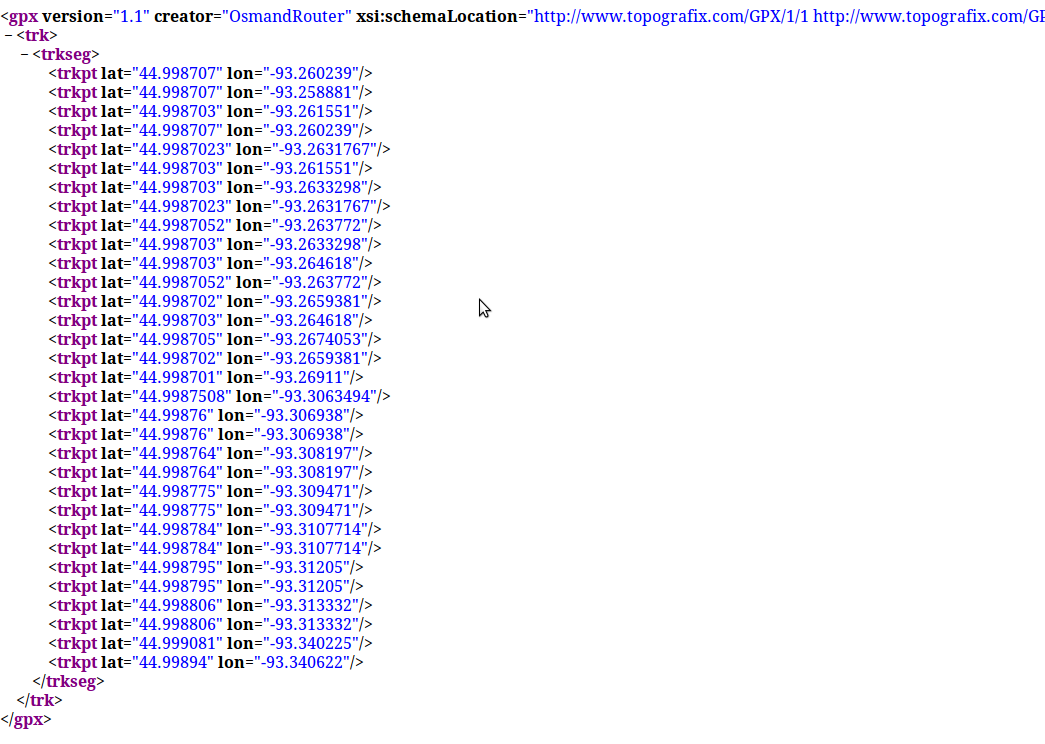
\includegraphics[scale=0.4]{gpx.png}
\caption{GPX file returned by the server}
\label{fig:gpx}
\end{minipage}
\centering
\end{figure}

Figure \ref{fig:gpx} is an example of a gpx file returned by the server. As it can be seen, the quickest path is represented by a set of coordinates. Our application then simply joins these points by straight lines which gives our quickest path.

\subsection{Server Side}
We used PostgreSQL\cite{postgressql} for storing the spatial data related to maps.  Currently we are focusing on the Minneapolis region of Minnesota USA. So, initially we got the openstreetmap for the Minneapolis region. This data was  in osm format which was xml. We used a tool called Osm2psql\cite{osm2psql}  to convert the  OpenStreetMap(.OSM) data into a format that can be loaded into PostgreSQL. For the support for geographic objects to the PostgreSQL object-relational database we used PostGIS\cite{postgis}. Actually PostGIS  spatially enables the PostgreSQL server, allowing it to be used as a backend spatial database for geographic information systems.\\

For calculating the shortest path we used another open source application called pgRouting\cite{pgrouting}. It actually extends the PostGIS/PostgreSQL geospatial database to provide geospatial routing functionality. PgRouting provides functions for

\begin{itemize}
\item Shortest Path Dijkstra
\item Shortest Path A-Star
\item Shortest Path Shooting-Star
\item Traveling Salesperson Problem(TSP)
\item Driving Distance calculation
\end{itemize}

In our current implementation, we are using Dijkstra algorithm for calculating the shortest route.


\subsubsection{Finding the corresponding edges the start and end points belong to}
\begin{figure}[H]
\begin{minipage}[b]{1.0\linewidth}
\centering
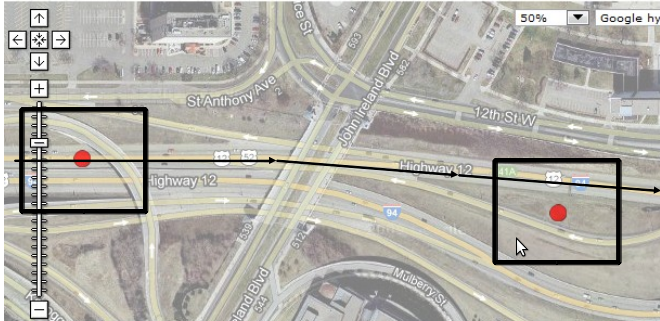
\includegraphics[scale=0.6]{start_end_edge.png}
\caption{Finding the corresponding edges of the start and end point}
\label{fig:start_end_edge}
\end{minipage}
\centering
\end{figure}

The first step in the server process is to actually find out the edge that the given start and end points belong to. For example in the figure given above the red circles denote the start and end points. However, they are off the edge. So the first thing to do is to find the edge that the points belong to. So what we do is create a bounding box around the circle and find the nearest edge for the points. Again pgRouting already provides this feature \cite{pgrouting_findedges}


\subsubsection{Maintaining information about the cost of edges and stations}

\begin{figure}[H]
\begin{minipage}[b]{1.0\linewidth}
\centering
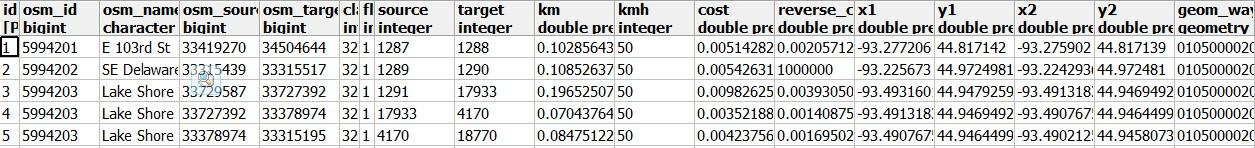
\includegraphics[scale=0.35]{edge_cost_information.jpg}
\caption{Database table containing edge details}
\label{fig:edge_cost_information}
\end{minipage}
\centering
\end{figure}

As you can see, the information about the edges is maintained in the database. Each edge has a unique osm id as well as the id given by the database. It has the information about the source and end vertex, their corresponding latitude and longitudes. Further, it has information about the speed limit in that edge given by the column kmh. The distance of the edge is given by the column km. Based upon these information we can calculate the cost of the edge given by the cost column. 

\begin{equation*}
speed = \frac{distance}{time}
\end{equation*}
\begin{equation*}
or,  cost=time=\frac{distance}{speed}
\end{equation*}

Hence the cost in our case is the time it requires to actually cover the length of the edge.
The information about the speed of traffic at a particular location is given  by speed sensors called stations. Since Minnesota Department of Transportation provides the station location (http://www.dot.state.mn.us/tmc/trafficinfo/developers.html), we use the same tools 3D box to find and manually connect the station id and edge id, which indicated as following image. Here we only used the main road station which contains 769 stations. An edge can even have more than one sensors associated with it. In this situation the speed of traffic at the edge will be the average of the sensors associated.

\begin{figure}[H]
\begin{minipage}[b]{1.0\linewidth}
\centering
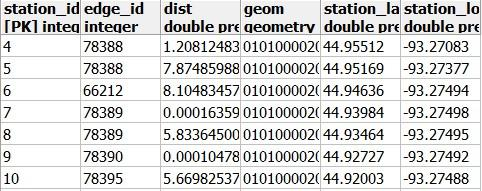
\includegraphics[scale=0.6]{station_edge.jpg}
\caption{Stations associated with edges}
\label{fig:station_edge}
\end{minipage}
\centering
\end{figure}

As you can see in figure \ref{fig:station_edge} a station is associated with an edge and multiple stations could be associated with an edge. The information given by the stations helps us to update the information regarding the traffic/speeds at different segments or edges. So, the idea is to regularly get the updates from the sensors, lets say a period of half an hour. From this information we can maintain records about the costs of edges at different interval.

\begin{figure}[H]
\begin{minipage}[b]{1.0\linewidth}
\centering
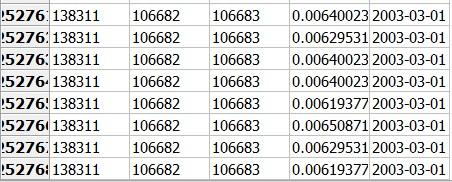
\includegraphics[scale=0.6]{edge_interval_cost.jpg}
\caption{Costs associated with edges at different interval}
\label{fig:edge_interval_cost}
\end{minipage}
\centering
\end{figure}

As you can see, we have the different cost information for the same edge at different time interval. One of the issues that we will face with this approach is that we will have lots of data eventually. So lets say  if we keep the records for the cost information every minute for an interval of 1 month, then it could easily consume lots of disk space. Furthermore, it would be time consuming to actually query the cost information from this huge table. Horizontal partitioning or indexing might help to resolve this issue. However, we propose that at any time we might not need to maintain all the cost information. Cost information of the recent 20-30 discrete intervals should be enough. At any time a person will be interested in the recent traffic information rather than the traffic information a year ago. So, we can actually archive the traffic information of the past and keep the fresh records in the production. Furthermore, a user may be interested in how the traffic will shape in the near future. This might help to answer his queries like if he needs to go from point A to point B, then will it be good for him to go now or after a period lets say half an hour. So our target will be to actually predict how the traffic will look like in that period. If it's less dense then it would be beneficial for him to move out later.\\

\small
\begin{table}[H]
\caption{Costs associated with edges}
\centering
\begin{tabular}{|>{\tiny}c |>{\tiny} c }
\hline
Cost of edges with station & Length/speed provided by sensor\\
Cost of edges without station: highway & Length)/speed limit\\
Cost of edges without station: local roads & Length/(20kmh) where 20 is default speed for local roads\\
\hline
\end{tabular}
\label{table:nonlin}
\end{table}

In the Minneapolis data we had the following stats regarding the edges and stations\\
Edges without stations = 180000\\
Edges with station = 769\\

\subsubsection{Getting the quickest path}

We used pgRouting's Dijsktra algorithm to calculate the quickest path. PgRouting actually provides special functions which we can query to get the quickest path. Further it allows us to specify the cost of the path. In our case it will be the time it takes to actually cover the path. As shown in the figure above, we can change the cost column, with that of the cost related to a particular time, lets say 30 minutes ago. So, now when pgRouting does the query to find the shortest path, it is based upon the traffic information 30 minutes ago. Further, we can maintain the cost information regarding the different edges at a different table and when making the actual query for the quickest path, we can pass the cost information for the edges from this separate table based upon the datetime information provided by the user.

\begin{figure}[H]
\begin{minipage}[b]{1.0\linewidth}
\centering
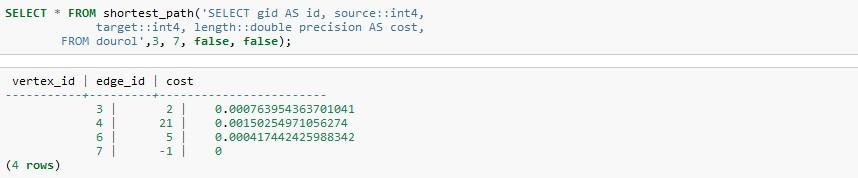
\includegraphics[scale=0.5]{shortest_path.jpg}
\caption{Calculating the quickest path}
\label{fig:quickest_path}
\end{minipage}
\centering
\end{figure}

Figure \ref{fig:quickest_path} shows the example of a query for a shortest path from the start node 3 and end node 7. The returned results shows that shortest path which consists of a list of edges and their corresponding cost. This means the person is to follow the path specified by the edges(which is the shortest) to actually reach his destination.\\

So, the basic algorithm to calculate the quickest path will be

\begin{itemize}
\item Based upon source and target point calculate the edge where the points belong to
\item Take the source vertex of the calculated starting edge as start node. Take the end vertex of the calculated ending edge as end node. 
\item Use the shortest\_path function provided by pgRouting to get the quickest path passing it the start and end node and the cost information of the edges based upon the date time information
\item Shortest\_path function returns the edges and their cost. From these edges calculate their corresponding start and end locations
\item Append the start and end locations of all the edges belonging to the shortest path into a gpx file
\item Return the gpx file to the client
\end{itemize}

\newpage
\begin{thebibliography}{50}
\bibitem{openstreetmap} http://www.openstreetmap.org/
\bibitem{android} http://developer.android.com/
\bibitem{osmand} http://osmand.net
\bibitem{openstreetmap_elements}http://wiki.openstreetmap.org/wiki/Elements
\bibitem{obf}http://wiki.openstreetmap.org/wiki/Elements
\bibitem{gpx} http://www.topografix.com/gpx.asp
\bibitem{postgressql} http://www.postgresql.org
\bibitem{osm2psql} http://wiki.openstreetmap.org/wiki/Osm2pgsql
\bibitem{postgis} http://postgis.refractions.net
\bibitem{pgrouting} http://www.pgrouting.org
\bibitem{pgrouting_findedges} http://workshop.pgrouting.org/chapters/php\_server.html
\end{thebibliography}

\end{document}



